% Plantilla de artículo inspirada en el formato de Applied Sciences (MDPI).
% Se usa desde compilar_pdf.py; el contenido proviene de TP1.md.
\documentclass[10pt,a4paper]{article}

\usepackage[a4paper,top=2.4cm,bottom=2.3cm,left=2.3cm,right=2.3cm,headsep=.55cm,footskip=.9cm]{geometry}
\usepackage{fontspec}
\setmainfont{TeX Gyre Pagella}
\setsansfont{TeX Gyre Heros}
\usepackage{polyglossia}
\setdefaultlanguage{spanish}
\usepackage{microtype}
\usepackage{graphicx,xcolor,array,calc,booktabs,longtable,multirow}
\usepackage{fancyhdr,lastpage,titlesec,enumitem,ragged2e}
\usepackage[font=small,labelformat=empty,skip=4pt,justification=justified,singlelinecheck=false]{caption}
\usepackage[hidelinks]{hyperref}

\definecolor{enlace}{HTML}{2F4F6F}
\hypersetup{colorlinks=true,linkcolor=enlace,urlcolor=enlace,citecolor=enlace}

% --- Párrafos -------------------------------------------------------------
\setlength{\parindent}{1.5em}
\setlength{\parskip}{0pt}
\linespread{1.05}
\setlength{\emergencystretch}{1.5em}
\providecommand{\tightlist}{\setlength{\itemsep}{0pt}\setlength{\parskip}{0pt}}
\setlist{leftmargin=2.2em,itemsep=1pt,topsep=3pt}
\setlist[enumerate]{label=\arabic*.}

\setcounter{secnumdepth}{0}
% --- Títulos de sección (MDPI: "1. Introducción" en negrita, subsecciones en itálica)
\titleformat{\section}{\normalfont\normalsize\bfseries}{}{0pt}{}
\titlespacing*{\section}{0pt}{10pt}{3pt}
\titleformat{\subsection}{\normalfont\normalsize\itshape}{}{0pt}{}
\titlespacing*{\subsection}{0pt}{7pt}{2pt}

% --- Encabezado y pie --------------------------------------------------------
\pagestyle{fancy}
\fancyhf{}
\fancyhead[L]{\small\itshape Aprendizaje Automático 2026 · TP1}
\fancyhead[R]{\small \thepage\ de \pageref*{LastPage}}
\renewcommand{\headrulewidth}{0.4pt}
\fancypagestyle{primera}{%
  \fancyhf{}
  \fancyfoot[L]{\small\itshape Aprendizaje Automático 2026 · TP1}
  \fancyfoot[R]{\small \thepage\ de \pageref*{LastPage}}
  \renewcommand{\headrulewidth}{0pt}
  \renewcommand{\footrulewidth}{0.4pt}}

% --- Figuras y tablas ---------------------------------------------------------
\setlength{\abovecaptionskip}{4pt}
\setlength{\textfloatsep}{10pt plus 2pt minus 2pt}
\setlength{\floatsep}{8pt plus 2pt minus 2pt}
\renewcommand{\topfraction}{.9}
\renewcommand{\bottomfraction}{.8}
\renewcommand{\textfraction}{.1}
\renewcommand{\floatpagefraction}{.8}
\newenvironment{tabla}{\par\begingroup\small
  \setlength{\LTpre}{2pt}\setlength{\LTpost}{2pt}\setlength{\tabcolsep}{4.5pt}
  \renewcommand{\arraystretch}{1.08}}{\endgroup\par}
\newcommand{\epigrafetabla}[1]{\noindent\begin{minipage}{\linewidth}\small\justifying\noindent #1\end{minipage}\par\vspace{2pt}}
\newcommand{\notatabla}[1]{\vspace{3pt}\noindent\begin{minipage}{\linewidth}\footnotesize\justifying\noindent #1\end{minipage}\par}
\setlength{\aboverulesep}{0pt}
\setlength{\belowrulesep}{0pt}
\renewcommand{\toprule}{\specialrule{1pt}{2pt}{2pt}}
\renewcommand{\bottomrule}{\specialrule{1pt}{2pt}{0pt}}
\renewcommand{\midrule}{\specialrule{.5pt}{2pt}{2pt}}

\begin{document}
\thispagestyle{primera}

\noindent{\small\itshape Artículo}\par\vspace{3pt}
\noindent{\LARGE\bfseries\raggedright Predicción de la deserción estudiantil: comparación de modelos de clasificación en una base
sintética\par}\vspace{8pt}
\noindent{\bfseries {[}completar{]}}\par\vspace{2pt}
\noindent{\small Trabajo práctico 1 --- Aprendizaje Automático, 2026}\par\vspace{12pt}

\noindent\begin{minipage}{\linewidth}
\setlength{\parindent}{1.5em}\small\justifying
\noindent\textbf{Resumen:} El objetivo de este trabajo fue comparar modelos de clasificación para predecir la deserción estudiantil, evaluar su
desempeño y capacidad de generalización. Se analizó una base sintética transformada de 50.000 registros y 27 predictores mediante clasificación
binaria ---Desertores frente a No desertores--- y multiclase ---Desertores, En Curso y Graduados---.\\
Los hiperparámetros se seleccionaron mediante validación cruzada en entrenamiento. La comparación principal utilizó todos los predictores, incluidos
los de ambos semestres. Como análisis adicional, se evaluó el aporte de incorporar sucesivamente información de inscripción y antecedentes, primer
semestre, segundo semestre y variables administrativas y familiares.\\
En los modelos binarios, Soft Voting obtuvo la mayor ROC-AUC (0,9514), apenas por encima de regresión logística (0,9506), sin mejorar su F1. En los
modelos multiclase, Random Forest alcanzó el mayor F1 macro (0,7808), mientras que En Curso fue la clase más difícil y se confundió principalmente con
Graduado. La mayor mejora predictiva apareció al incorporar el primer semestre.\\
Los resultados muestran capacidad predictiva exploratoria en esta base. La exploración previa del test limita la evaluación, y el uso de información
de ambos semestres no demuestra anticipación del abandono desde la inscripción.
\par\vspace{6pt}
\noindent\textbf{Palabras clave:} deserción estudiantil; aprendizaje automático; clasificación multiclase; validación cruzada; importancia por
permutación
\end{minipage}
\par\vspace{6pt}\noindent\rule{\linewidth}{0.4pt}\vspace{2pt}

\hypertarget{introducciuxf3n}{%
\section{1. Introducción}\label{introducciuxf3n}}

La predicción de la deserción estudiantil mediante aprendizaje automático permite evaluar la utilidad de los registros institucionales para reconocer
estudiantes en riesgo {[}1{]}. Este trabajo examina esa capacidad predictiva mediante dos tareas: distinguir Desertor de No desertor y diferenciar los
estados Desertor, En Curso y Graduado. Se compararon modelos de clasificación y se analizó el aporte de la información académica, administrativa y de
ingreso.

Los antecedentes destacan la relevancia del rendimiento académico y de las condiciones financieras. Delen {[}1{]}, a partir de ocho años de datos
institucionales, identificó ambos grupos entre los predictores más importantes. En el Instituto Politécnico de Portalegre, Portugal, Realinho et
al.~{[}2{]} encontraron cinco predictores relevantes en los cuatro algoritmos examinados: materias aprobadas de ambos semestres, nota del segundo
semestre, carrera y matrícula al día. Sobre esta fuente, Martins et al.~{[}3{]} compararon distintas etapas del primer año: el mayor F1 global
reportado pasó de 0,650 con información de inscripción a 0,745 al incorporar el primer semestre.

Estos antecedentes motivaron el análisis de una versión sintética y transformada de esa fuente {[}4{]}. El objetivo fue comparar el desempeño y
examinar la capacidad de generalización de los modelos, así como identificar qué información contribuyó a sus predicciones. Se utilizaron todos los
predictores y, como análisis adicional, se incorporaron grupos de variables de forma acumulativa. A partir de los antecedentes y de la exploración en
entrenamiento se formularon tres hipótesis exploratorias:

\begin{itemize}
\tightlist
\item
  La actividad y el rendimiento académico del primer año aportan la mayor información predictiva \textbf{(H1)}.
\item
  Las variables administrativas y de ingreso aportan información, pero menos que las académicas \textbf{(H2)}.
\item
  En Curso presenta menor sensibilidad y F1 que las otras clases y se confunde principalmente con Graduado; agrupar ambas como No desertor oculta esa
  confusión \textbf{(H3)}.
\end{itemize}

\hypertarget{materiales-y-muxe9todos}{%
\section{2. Materiales y métodos}\label{materiales-y-muxe9todos}}

\hypertarget{datos-y-variables-explicativas}{%
\subsection{2.1. Datos y variables explicativas}\label{datos-y-variables-explicativas}}

Se utilizó el archivo \texttt{dataset\_TP1\_2026.csv}, con 50.000 registros, 27 predictores y una variable respuesta. La base procede de Kaggle
Playground Series S4E6 {[}4{]}, un conjunto sintético derivado de \emph{Predict Students' Dropout and Academic Success} {[}2{]}. El script de
preparación disponible {[}5{]} documenta traducciones, agrupamientos, reescalados y muestreo por respuesta y carrera. El presente análisis utilizó el
archivo ya preparado, cuyos nombres y categorías están en castellano.

Los 11 predictores numéricos y 16 categóricos se organizaron en cuatro grupos (Tabla 1). Se desconoce la fecha de registro o actualización del grupo
administrativo y familiar. Los rótulos de ingresos y demanda cognitiva son recodificaciones de ocupación.

\begin{table}[!htbp]
\begin{tabla}
\epigrafetabla{\textbf{Tabla 1.} Grupos de predictores. La comparación principal
incluyó las 27 variables; el análisis acumulativo (Sección 2.5) agregó
los grupos en el orden de la tabla.}
\begin{tabular*}{\linewidth}{@{\extracolsep{\fill}}
  >{\raggedright\arraybackslash}p{(\columnwidth - 6\tabcolsep) * \real{0.1746}}
  >{\raggedright\arraybackslash}p{(\columnwidth - 6\tabcolsep) * \real{0.5397}}
  >{\raggedright\arraybackslash}p{(\columnwidth - 6\tabcolsep) * \real{0.1746}}
  >{\raggedleft\arraybackslash}p{(\columnwidth - 6\tabcolsep) * \real{0.1111}}@{}}
\toprule\noalign{}
\begin{minipage}[b]{\linewidth}\raggedright
Grupo
\end{minipage} & \begin{minipage}[b]{\linewidth}\raggedright
Variables
\end{minipage} & \begin{minipage}[b]{\linewidth}\raggedright
Tipo
\end{minipage} & \begin{minipage}[b]{\linewidth}\raggedleft
Acumulado
\end{minipage} \\
\midrule\noalign{}
Inscripción y antecedentes & Estudios previos, nota de estudios previos,
puntaje de ingreso, modo de acceso, carrera, turno, edad al inscribirse,
sexo, estado civil, desplazamiento, estudiante internacional,
necesidades educativas especiales & 9 categóricas, 3 numéricas & 12 \\
Primer semestre (S1) & Materias inscriptas, evaluaciones, materias
aprobadas, nota promedio & 4 numéricas & 16 \\
Segundo semestre (S2) & Las mismas cuatro medidas del segundo semestre &
4 numéricas & 20 \\
Administrativas y familiares & Deuda, matrícula al día, beca, ingresos y
demanda cognitiva de la ocupación de cada progenitor & 7 categóricas &
27 \\
\bottomrule
\end{tabular*}
\notatabla{El grupo administrativo y familiar no representa una etapa posterior a
S2: se incorporó al final porque su fecha de disponibilidad es
desconocida.}
\end{tabla}
\end{table}

El análisis exploratorio se realizó en el entrenamiento de la partición multiclase: 18.966 registros Graduado (47,42 \%), 13.223 Desertor (33,06 \%) y
7.811 En Curso (19,53 \%). El desbalance se consideró en la evaluación mediante F1 macro y métricas por clase; no se aplicaron remuestreo ni pesos de
clase al entrenamiento.

En este conjunto no se detectaron faltantes explícitos. Se conservaron 213 repeticiones de filas completas y 235 repeticiones de perfiles de
predictores; 22 perfiles presentaban etiquetas diferentes. También se conservaron 34 casos de S1 y 62 de S2 con más materias aprobadas que inscriptas,
por falta de información para corregirlos. Dos pares de variables parentales eran recodificaciones equivalentes. Los ceros académicos se analizaron
por separado y no se trataron como faltantes.

\hypertarget{variable-respuesta-y-particiones}{%
\subsection{2.2. Variable respuesta y particiones}\label{variable-respuesta-y-particiones}}

La tarea binaria definió Desertor como clase positiva (1) y agrupó En Curso y Graduado como No desertor (0). La tarea multiclase conservó las tres
etiquetas. En Curso representa un estado observado, sin información sobre la trayectoria posterior.

Cada tarea utilizó una partición estratificada por su propia respuesta, con 80 \% para entrenamiento (40.000 registros), 20 \% para prueba (10.000) y
semilla 42. Las particiones binarias y multiclase no contienen exactamente los mismos registros. Una exploración previa había examinado las etiquetas
de toda la base; por ello, el conjunto de prueba no constituye una evaluación independiente y sus resultados se consideran exploratorios.

\hypertarget{preprocesamiento-y-modelos}{%
\subsection{2.3. Preprocesamiento y modelos}\label{preprocesamiento-y-modelos}}

El análisis se implementó en Python con scikit-learn. La comparación principal incluyó los 27 predictores. El preprocesamiento y el clasificador se
integraron en un \emph{pipeline}, ajustado dentro de cada partición de entrenamiento de la validación cruzada. Se incluyeron imputadores por mediana y
moda, que no reemplazaron valores por ausencia de faltantes. La codificación \emph{one-hot} de las variables categóricas, junto con las numéricas,
produjo 77 columnas. Las numéricas se estandarizaron para regresión logística, SVM y K-NN. Se conservaron todos los predictores.

En la tarea binaria se compararon regresión logística con penalización L2, máquinas de soporte vectorial con núcleo RBF (SVM) y árboles de decisión
con criterio Gini. La regresión logística transforma una combinación lineal de predictores en una probabilidad mediante la función logística; L2
limita la magnitud de sus coeficientes. SVM RBF admite fronteras no lineales, mientras que el árbol representa interacciones mediante divisiones
sucesivas. Su complejidad se controló mediante los hiperparámetros de la Tabla 2.

En multiclase se evaluaron K-NN, árboles de decisión, Random Forest (RF) y AdaBoost. K-NN determina la clase a partir de los vecinos más próximos. RF
combina árboles entrenados con muestras \emph{bootstrap} y selección aleatoria de variables en cada división, una estrategia orientada a reducir la
varianza {[}6{]}; se fijó \texttt{max\_features="sqrt"}. AdaBoost combina árboles pequeños de forma secuencial, aumentando el peso de los casos mal
clasificados. Estos modelos admiten directamente las tres clases.

\hypertarget{selecciuxf3n-de-hiperparuxe1metros-y-evaluaciuxf3n}{%
\subsection{2.4. Selección de hiperparámetros y evaluación}\label{selecciuxf3n-de-hiperparuxe1metros-y-evaluaciuxf3n}}

Para cada modelo se definió una grilla de valores candidatos (Tabla 2). Todas sus combinaciones se evaluaron mediante validación cruzada estratificada
de tres particiones (\emph{folds}) dentro de entrenamiento. En cada iteración se utilizaron aproximadamente 26.667 registros para ajustar y 13.333
para validar. Se eligió la configuración con mayor ROC-AUC media en binario o mayor F1 macro medio en multiclase; luego se reajustó con los 40.000
registros y se evaluó en prueba.

\begin{table}[!htbp]
\begin{tabla}
\epigrafetabla{\textbf{Tabla 2.} Hiperparámetros evaluados y configuraciones
seleccionadas mediante validación cruzada.}
\begin{tabular*}{\linewidth}{@{\extracolsep{\fill}}lll@{}}
\toprule\noalign{}
Tarea · modelo & Valores probados & Elegido \\
\midrule\noalign{}
Binaria · Logística & C: 0,01; 0,1; 1; 10 & C=0,1 \\
Binaria · SVM & C: 0,1; 1; 10 · γ: scale; 0,01; 0,1 & C=0,1; γ=0,01 \\
Binaria · Árbol & profundidad: 2; 4; 6; 8; 12; sin límite · hoja mín.:
1; 10; 50 & prof. 8; hoja 50 \\
3 clases · K-NN & k: 3; 5; 9; 15; 25 · peso: uniforme, distancia & k=25;
uniforme \\
3 clases · Árbol & profundidad: 2; 4; 6; 8; 12; sin límite · hoja mín.:
1; 10; 50 & prof. 12; hoja 50 \\
3 clases · Random Forest & árboles: 200; 500 · profundidad: 12, sin
límite · hoja mín.: 1; 50 & 500; sin límite; hoja 1 \\
3 clases · AdaBoost & prof. base: 1; 2 · árboles: 100; 200; 400 · tasa:
0,05; 0,1 & prof. 2; 400; tasa 0,1 \\
\bottomrule
\end{tabular*}
\notatabla{C es la inversa de la intensidad de regularización; γ, el parámetro del
núcleo RBF; k, la cantidad de vecinos; hoja mín., el mínimo de casos por
hoja.}
\end{tabla}
\end{table}

Se construyó un ensamble Soft Voting con los tres modelos binarios seleccionados, promediando sus probabilidades con pesos iguales. Las probabilidades
del SVM se obtuvieron mediante calibración sigmoide del pipeline completo con \texttt{CalibratedClassifierCV}, tres folds internos y
\texttt{ensemble=False}. Esta validación interna se utilizó para calibrar probabilidades y fue distinta de la búsqueda de hiperparámetros.

Se calcularon accuracy, precisión, sensibilidad (\emph{recall}), F1 y ROC-AUC. F1 combina precisión y sensibilidad; ROC-AUC evalúa la discriminación
entre clases a distintos umbrales. En binario, precisión, sensibilidad y F1 se calcularon para Desertor. En multiclase se utilizaron promedios macro,
que asignan igual peso a cada clase al evaluar; la AUC se calculó comparando cada clase frente al resto (OvR) y promediando sus valores. Las
predicciones probabilísticas asignaron la clase más probable; el SVM individual utilizó el signo de su función de decisión.

\hypertarget{anuxe1lisis-complementarios}{%
\subsection{2.5. Análisis complementarios}\label{anuxe1lisis-complementarios}}

El aporte de los grupos de variables se estudió mediante regresión logística binaria y árbol multiclase. Se incorporaron sucesivamente inscripción y
antecedentes (12 predictores), S1 (16), S2 (20) y variables administrativas y familiares (27). Se mantuvieron las filas y los folds dentro de cada
tarea, seleccionando hiperparámetros en cada etapa. La comparación evalúa el desempeño alcanzado con cada conjunto de información y no aísla el efecto
de agregar variables a una configuración fija. En ambas tareas se utilizó la partición estratificada por tres clases, distinta de la partición binaria
principal.

Se construyeron curvas de complejidad comparando entrenamiento y validación al variar un hiperparámetro. Por costo computacional, las curvas de RF y
AdaBoost utilizaron 12.000 registros y la de K-NN, 6.000. Se incluyó una referencia Dummy que predice la clase mayoritaria, se compararon tres y cinco
folds con configuraciones fijas y se realizó una segunda búsqueda para el árbol. Las ampliaciones de las grillas de K-NN y AdaBoost se efectuaron
después de observar el conjunto de prueba y no modificaron los modelos finales.

La importancia de variables se estimó mediante la caída del F1 macro de RF al permutar cada predictor original antes de \emph{one-hot}, con cinco
repeticiones por variable en cada uno de tres folds de validación. Finalmente, se recalcularon las métricas del análisis acumulativo excluyendo del
conjunto de prueba los perfiles idénticos a los de entrenamiento, sin reajustar los modelos.

\hypertarget{resultados}{%
\section{3. Resultados}\label{resultados}}

\hypertarget{caracteruxedsticas-de-las-clases}{%
\subsection{3.1. Características de las clases}\label{caracteruxedsticas-de-las-clases}}

La proporción de registros sin materias aprobadas fue mayor en Desertor: 58,1 \% en S1 y 67,9 \% en S2, frente a 4,2 \% y 4,6 \% en En Curso y
aproximadamente 1,5 \% en Graduado para ambos semestres (Figura 1a). Entre quienes aprobaron al menos una materia, las medianas para Desertor, En
Curso y Graduado fueron, respectivamente, 4, 5 y 6 en S1, y 3, 4 y 6 en S2. La ausencia de aprobaciones no permite distinguir entre no rendir y rendir
sin aprobar.

La proporción de Desertor fue 93,79 \% entre quienes no tenían la matrícula al día (n=4.332), 76,05 \% entre quienes tenían deuda (n=2.877) y 7,21 \%
entre quienes tenían beca (n=9.930), frente al 33,06 \% del entrenamiento completo (Figura 1b). La mediana de edad fue 22 años en Desertor y 19 en las
otras clases.

\begin{figure}[!htbp]
\centering
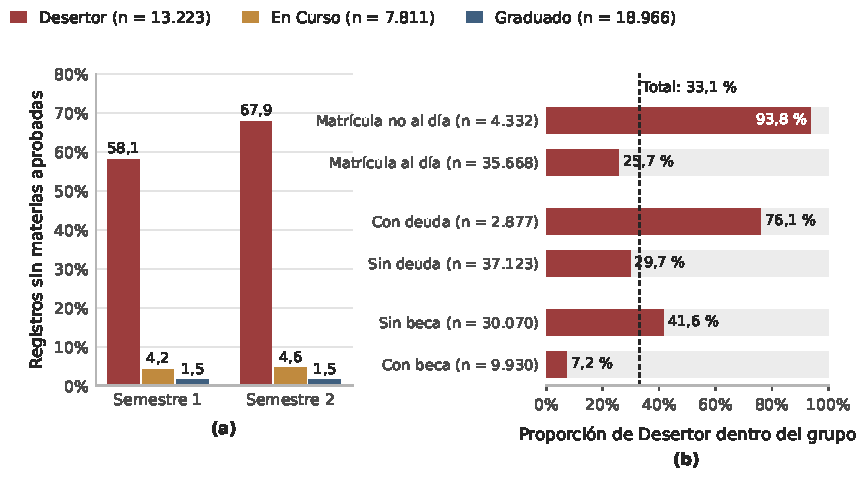
\includegraphics[width=\linewidth]{figuras/figura_01.pdf}
\caption*{\textbf{Figura 1.} Asociaciones exploratorias en entrenamiento
(n=40.000): (\textbf{a}) porcentaje de registros sin materias aprobadas
dentro de cada clase, por semestre; (\textbf{b}) proporción de Desertor
dentro de cada grupo administrativo; la línea discontinua indica la
proporción en todo el entrenamiento. Cada porcentaje utiliza como
denominador su propio grupo.}
\end{figure}

\hypertarget{clasificaciuxf3n-binaria}{%
\subsection{3.2. Clasificación binaria}\label{clasificaciuxf3n-binaria}}

La regresión logística obtuvo el mayor F1 (0,8510). Soft Voting alcanzó la mayor ROC-AUC (0,9514), frente a 0,9506 de regresión logística, pero
presentó menor sensibilidad y F1 (Tabla 3). En los tres modelos individuales, la AUC de prueba difirió en 0,0005 o menos de la media de validación
cruzada.

\begin{table}[!htbp]
\begin{tabla}
\epigrafetabla{\textbf{Tabla 3.} Desempeño de los modelos binarios en validación
cruzada (media ± DE de tres folds en entrenamiento) y en prueba
(n=10.000). La negrita indica el mejor valor de cada columna.}
\begin{tabular*}{\linewidth}{@{\extracolsep{\fill}}lrrrrrr@{}}
\toprule\noalign{}
Modelo & ROC-AUC validación & Accuracy & Precisión & Sensibilidad & F1 &
ROC-AUC \\
\midrule\noalign{}
Logística & \textbf{0,9507 ± 0,0013} & \textbf{0,9066} & 0,9004 &
\textbf{0,8067} & \textbf{0,8510} & 0,9506 \\
SVM & 0,9462 ± 0,0012 & 0,8979 & \textbf{0,9150} & 0,7619 & 0,8315 &
0,9460 \\
Árbol & 0,9445 ± 0,0016 & 0,9057 & 0,9064 & 0,7970 & 0,8482 & 0,9440 \\
Soft Voting & --- & 0,9053 & 0,9080 & 0,7940 & 0,8472 &
\textbf{0,9514} \\
\bottomrule
\end{tabular*}
\notatabla{Precisión, sensibilidad y F1 corresponden a Desertor. Accuracy
representa la proporción total de aciertos; precisión, la proporción de
desertores entre los casos señalados; sensibilidad, la proporción
detectada entre los desertores reales. ROC-AUC: área bajo la curva ROC.
Soft Voting no se seleccionó por validación cruzada. La DE describe la
variación entre folds y no es un intervalo de confianza.}
\end{tabla}
\end{table}

Las curvas ROC de los cuatro modelos se superpusieron en casi todo su recorrido (Figura 2a). Con el corte por defecto, los modelos se ubicaron en una
región similar de la curva; SVM mostró menor sensibilidad con menor proporción de falsos positivos (Figura 2b).

\begin{figure}[!htbp]
\centering
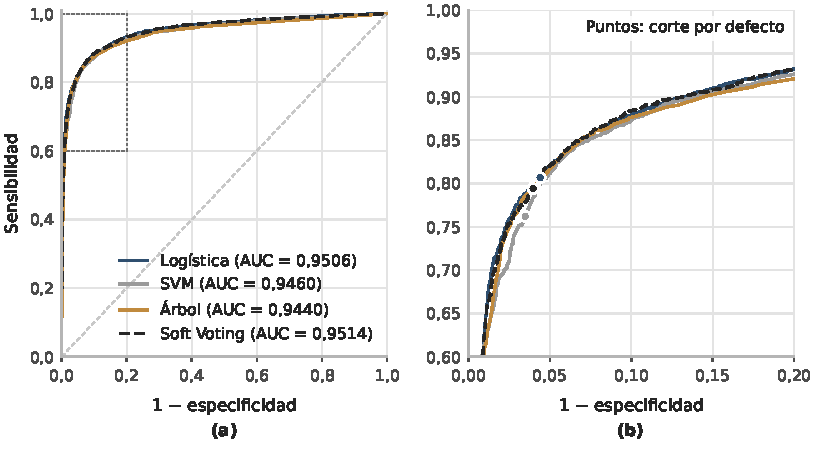
\includegraphics[width=\linewidth]{figuras/figura_02.pdf}
\caption*{\textbf{Figura 2.} Curvas ROC de los modelos binarios en prueba
(n=10.000): (\textbf{a}) curvas completas; la diagonal corresponde a una
clasificación sin discriminación; (\textbf{b}) detalle del recuadro de
(a). Los puntos indican el corte por defecto: probabilidad 0,5 o signo
de la función de decisión en SVM.}
\end{figure}

\hypertarget{clasificaciuxf3n-multiclase}{%
\subsection{3.3. Clasificación multiclase}\label{clasificaciuxf3n-multiclase}}

RF obtuvo el mayor F1 macro (0,7808), seguido por AdaBoost (0,7776), árbol (0,7699) y K-NN (0,7483) (Tabla 4).

\begin{table}[!htbp]
\begin{tabla}
\epigrafetabla{\textbf{Tabla 4.} Desempeño de los modelos multiclase en validación
cruzada (media ± DE de tres folds en entrenamiento) y en prueba
(n=10.000). La negrita indica el mejor valor de cada columna.}
\begin{tabular*}{\linewidth}{@{\extracolsep{\fill}}lrrrrrr@{}}
\toprule\noalign{}
Modelo & F1 macro validación & Accuracy & Precisión macro & Sensibilidad
macro & F1 macro & ROC-AUC OvR \\
\midrule\noalign{}
K-NN & 0,7487 ± 0,0035 & 0,7943 & 0,7664 & 0,7388 & 0,7483 & 0,9034 \\
Árbol & 0,7698 ± 0,0041 & 0,8106 & 0,7774 & 0,7647 & 0,7699 & 0,9170 \\
Random Forest & \textbf{0,7814 ± 0,0008} & \textbf{0,8196} &
\textbf{0,7896} & \textbf{0,7750} & \textbf{0,7808} & \textbf{0,9254} \\
AdaBoost & 0,7715 ± 0,0038 & 0,8182 & 0,7874 & 0,7707 & 0,7776 &
0,9219 \\
\bottomrule
\end{tabular*}
\notatabla{Los promedios macro asignan igual peso a las tres clases. ROC-AUC OvR
corresponde al promedio macro de las comparaciones de cada clase frente
al resto.}
\end{tabla}
\end{table}

En Curso presentó el menor F1 en los cuatro modelos (Tabla 5). En RF, su sensibilidad fue 0,5981, frente a 0,8076 para Desertor y 0,9192 para
Graduado. El mayor F1 de Desertor correspondió a AdaBoost (0,8562).

\begin{table}[!htbp]
\begin{tabla}
\epigrafetabla{\textbf{Tabla 5.} F1 de cada clase en prueba (n=10.000). La negrita
indica el mejor valor de cada columna.}
\begin{tabular*}{\linewidth}{@{\extracolsep{\fill}}lrrrr@{}}
\toprule\noalign{}
Modelo & F1 macro & Desertor (n=3.306) & En Curso (n=1.953) & Graduado
(n=4.741) \\
\midrule\noalign{}
K-NN & 0,7483 & 0,8306 & 0,5542 & 0,8602 \\
Árbol & 0,7699 & 0,8472 & 0,5899 & 0,8726 \\
Random Forest & \textbf{0,7808} & 0,8529 & \textbf{0,6096} &
\textbf{0,8798} \\
AdaBoost & 0,7776 & \textbf{0,8562} & 0,6006 & 0,8758 \\
\bottomrule
\end{tabular*}
\notatabla{Entre paréntesis, número de registros de cada clase en prueba.}
\end{tabla}
\end{table}

En los cuatro modelos, la mayor parte de los errores en En Curso correspondió a predicciones de Graduado (entre 29 \% y 39 \% de la clase; Figura 3).
De los 1.953 registros En Curso, RF clasificó 569 (29,1 \%) como Graduado y 216 (11,1 \%) como Desertor. La primera confusión queda oculta al agrupar
En Curso y Graduado en una única categoría. Esta propiedad de las etiquetas no equivale al resultado de entrenar un clasificador binario.

\begin{figure}[!htbp]
\centering
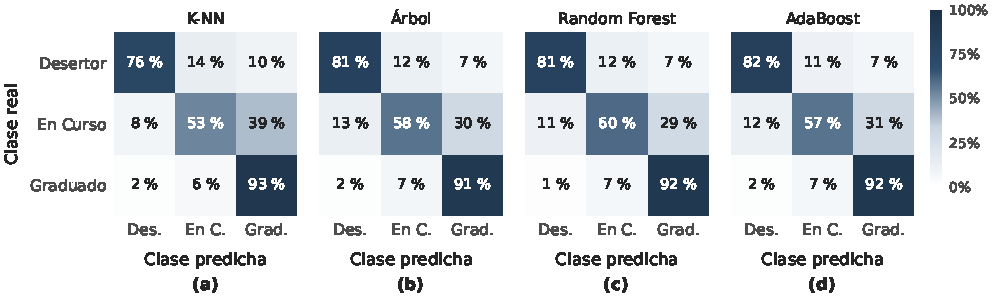
\includegraphics[width=\linewidth]{figuras/figura_03.pdf}
\caption*{\textbf{Figura 3.} Matrices de confusión en prueba (n=10.000) para
(\textbf{a}) K-NN, (\textbf{b}) árbol, (\textbf{c}) Random Forest y
(\textbf{d}) AdaBoost. Cada fila presenta el porcentaje de una clase
real asignado a cada clase predicha y suma 100 \%. Des.: Desertor; En
C.: En Curso; Grad.: Graduado.}
\end{figure}

\hypertarget{complejidad-y-generalizaciuxf3n}{%
\subsection{3.4. Complejidad y generalización}\label{complejidad-y-generalizaciuxf3n}}

En la tarea binaria, la AUC de validación de regresión logística varió poco entre C=0,01 y 10 (aproximadamente 0,9504--0,9507). En SVM, aumentar C
desde la mejor región ensayada redujo el desempeño de validación. En el árbol con hoja mínima de 50 registros, la AUC alcanzó 0,9445 en profundidad 8
y luego se estabilizó, mientras el desempeño de entrenamiento continuó aumentando (Figura 4).

\begin{figure}[!htbp]
\centering
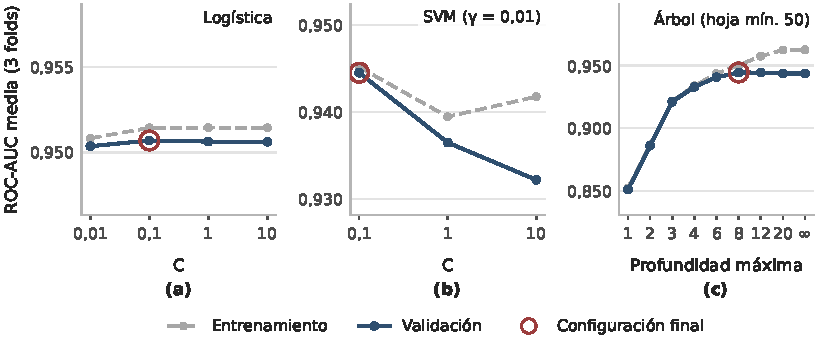
\includegraphics[width=\linewidth]{figuras/figura_04.pdf}
\caption*{\textbf{Figura 4.} Curvas de complejidad de los modelos binarios:
ROC-AUC media de entrenamiento y validación en tres folds sobre 40.000
registros para (\textbf{a}) regresión logística según C; (\textbf{b})
SVM según C con γ=0,01; (\textbf{c}) árbol según la profundidad máxima
con hoja mínima de 50 registros. El círculo marca la configuración
final. Las escalas verticales difieren entre paneles.}
\end{figure}

En multiclase, el RF reducido aumentó su F1 macro de validación de 0,7294 a 0,7741 entre profundidades 4 y 12; sin límite alcanzó 0,7738. Esta curva
utilizó 80 árboles y hoja mínima de 10 registros, una configuración distinta de la final. K-NN con k=3 obtuvo 0,823 en entrenamiento y 0,700 en
validación; el mayor valor de la curva se observó en k=11. La búsqueda principal seleccionó k=25 con otra muestra y otros candidatos. AdaBoost aumentó
de 0,7656 a 0,7771 entre 100 y 600 árboles, sin descenso en el rango evaluado (Figura 5).

\begin{figure}[!htbp]
\centering
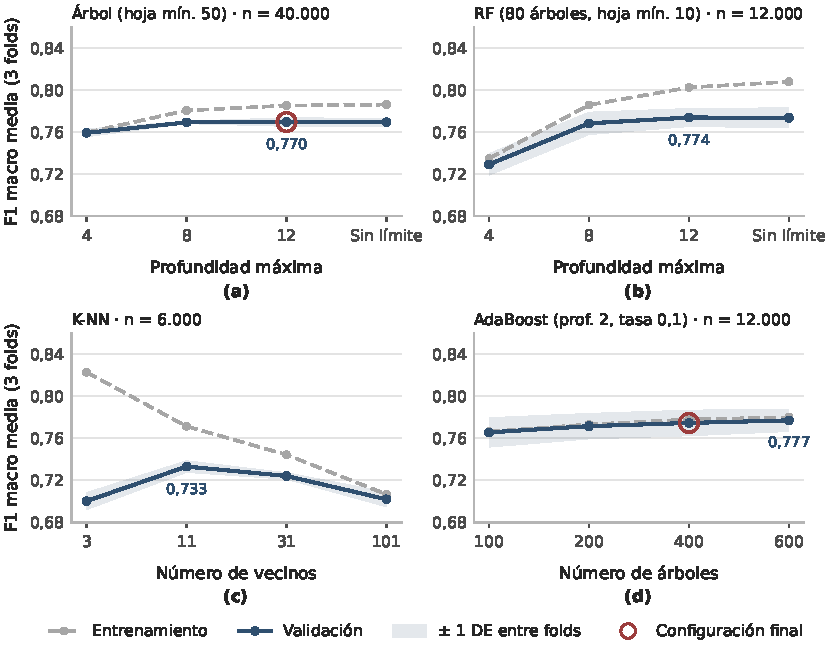
\includegraphics[width=\linewidth]{figuras/figura_05.pdf}
\caption*{\textbf{Figura 5.} Curvas de complejidad de los modelos multiclase: F1
macro medio de entrenamiento y validación en tres folds para
(\textbf{a}) árbol, 40.000 registros; (\textbf{b}) RF reducido, 12.000;
(\textbf{c}) K-NN, 6.000; (\textbf{d}) AdaBoost, 12.000. La banda indica
± 1 DE entre folds de validación y el número, el máximo de validación de
cada curva. El círculo marca el valor de la configuración final cuando
la curva lo incluye. Cada curva corresponde a su propio protocolo.}
\end{figure}

\hypertarget{referencia-y-sensibilidad-de-la-selecciuxf3n}{%
\subsection{3.5. Referencia y sensibilidad de la selección}\label{referencia-y-sensibilidad-de-la-selecciuxf3n}}

La referencia Dummy obtuvo ROC-AUC 0,500 en binario y F1 macro 0,214 en multiclase, por debajo de todos los modelos y aun de los entrenados solo con
las variables de inscripción (Figura 6).

Con configuraciones fijas, el cambio de tres a cinco folds modificó la AUC de regresión logística de 0,9503 a 0,9505 y el F1 macro del árbol de 0,7698
a 0,7690. En RF reducido, con 80 árboles, profundidad 12 y hoja mínima 10, cambió de 0,7741 a 0,7726. Esta comparación utilizó la partición
estratificada por tres clases y no repitió la búsqueda completa de hiperparámetros. Ninguno de estos cambios superó la DE entre los tres folds de la
misma configuración (0,0002 en regresión logística, 0,0041 en árbol y 0,0086 en RF).

En la segunda grilla del árbol, profundidad 12 y hoja mínima 50 alcanzó F1 macro de validación 0,7698, frente a 0,7694 con profundidad 8 y la misma
hoja. Sin límite de profundidad y con hoja mínima 10, el F1 macro fue 0,8250 en entrenamiento y 0,7446 en validación.

La ampliación de las grillas no mejoró K-NN más allá de 25 vecinos, mientras que AdaBoost continuó mejorando hasta 600 árboles (Tabla 6). Estas
comprobaciones posteriores no modificaron las configuraciones finales.

\begin{table}[!htbp]
\begin{tabla}
\epigrafetabla{\textbf{Tabla 6.} Ampliación de grillas: F1 macro medio en validación de
tres folds sobre 40.000 registros. La negrita indica el mayor valor de
cada modelo.}
\begin{tabular*}{\linewidth}{@{\extracolsep{\fill}}lllrr@{}}
\toprule\noalign{}
Modelo & Configuración fija & Hiperparámetro & Valor & F1 macro \\
\midrule\noalign{}
K-NN & pesos uniformes & \emph{k} (n.º de vecinos) & 25 &
\textbf{0,7487} \\
& & & 35 & 0,7475 \\
& & & 51 & 0,7453 \\
AdaBoost & profundidad 2; tasa 0,1 & n.º de árboles & 200 & 0,7623 \\
& & & 400 & 0,7715 \\
& & & 600 & \textbf{0,7747} \\
\bottomrule
\end{tabular*}
\end{tabla}
\end{table}

\hypertarget{aporte-acumulativo-de-los-grupos-de-variables}{%
\subsection{3.6. Aporte acumulativo de los grupos de variables}\label{aporte-acumulativo-de-los-grupos-de-variables}}

La incorporación de S1 a las 12 variables de inscripción y antecedentes aumentó la AUC de validación de regresión logística de 0,7941 a 0,9262. Al
agregar S2 se alcanzó 0,9422 y, con las variables administrativas y familiares, 0,9503. En el árbol multiclase, los valores de F1 macro fueron 0,5603,
0,7115, 0,7529 y 0,7698, respectivamente (Figura 6). En ambas tareas, el mayor incremento se observó al incorporar S1.

\begin{figure}[!htbp]
\centering
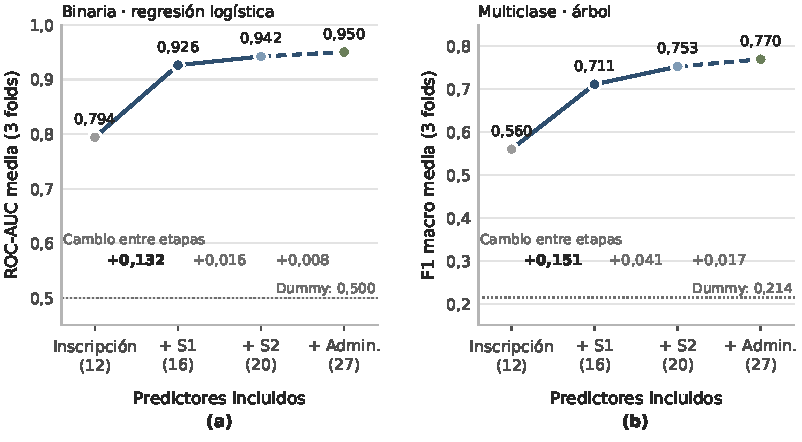
\includegraphics[width=\linewidth]{figuras/figura_06.pdf}
\caption*{\textbf{Figura 6.} Desempeño en validación cruzada del análisis
acumulativo: (\textbf{a}) ROC-AUC de regresión logística binaria;
(\textbf{b}) F1 macro del árbol multiclase. Se incorporaron
sucesivamente 12, 16, 20 y 27 predictores (Tabla 1), manteniendo las
filas y los folds dentro de cada tarea y seleccionando hiperparámetros
en cada etapa. Los números inferiores indican el cambio entre etapas
consecutivas. El tramo discontinuo incorpora el grupo administrativo y
familiar, cuya fecha de disponibilidad es desconocida. La línea punteada
indica la referencia Dummy.}
\end{figure}

\hypertarget{importancia-de-los-predictores}{%
\subsection{3.7. Importancia de los predictores}\label{importancia-de-los-predictores}}

Las mayores caídas del F1 macro de RF por permutación correspondieron a materias aprobadas en S2 (0,1004) y matrícula al día (0,0360) (Figura 7). Las
sumas descriptivas de importancias positivas fueron 0,1533 para las ocho variables académicas, 0,0468 para deuda, matrícula y beca, y 0,0075 para las
otras 16 variables. Estas sumas no equivalen a permutar grupos completos ni descomponen el desempeño del modelo.

\begin{figure}[!htbp]
\centering
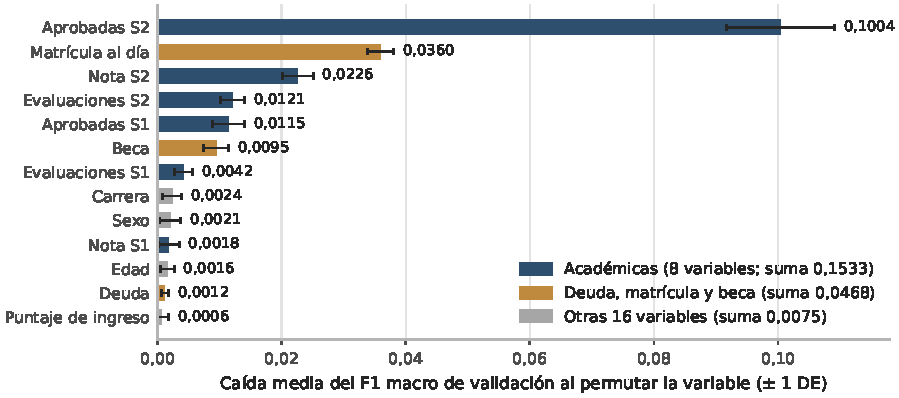
\includegraphics[width=\linewidth]{figuras/figura_07.pdf}
\caption*{\textbf{Figura 7.} Importancia por permutación en RF: caída media del F1
macro de validación al permutar cada predictor original (± 1 DE). Se
muestran las 13 variables con mayor caída, coloreadas según el grupo
utilizado en las sumas descriptivas. Un valor mayor indica mayor
dependencia predictiva del modelo respecto de esa variable.}
\end{figure}

\hypertarget{sensibilidad-a-los-perfiles-repetidos}{%
\subsection{3.8. Sensibilidad a los perfiles repetidos}\label{sensibilidad-a-los-perfiles-repetidos}}

En el análisis acumulativo, 103 registros de prueba compartían los mismos 27 predictores con alguna fila de entrenamiento; en 94 también coincidía la
etiqueta. Al excluirlos sin reajustar los modelos, las métricas disminuyeron entre 0,0005 y 0,0007 (Tabla 7).

\begin{table}[!htbp]
\begin{tabla}
\epigrafetabla{\textbf{Tabla 7.} Desempeño de los modelos del análisis acumulativo con
y sin perfiles repetidos en prueba.}
\begin{tabular*}{\linewidth}{@{\extracolsep{\fill}}llrr@{}}
\toprule\noalign{}
Modelo & Métrica & Test completo (n=10.000) & Sin repetidos (n=9.897) \\
\midrule\noalign{}
Logística binaria, 20 variables & ROC-AUC & 0,9446 & 0,9440 \\
Árbol multiclase, 20 variables & F1 macro & 0,7455 & 0,7448 \\
Logística binaria, 27 variables & ROC-AUC & 0,9518 & 0,9513 \\
Árbol multiclase, 27 variables & F1 macro & 0,7699 & 0,7694 \\
\bottomrule
\end{tabular*}
\notatabla{Las métricas se recalcularon sin reentrenamiento. La AUC 0,9518
corresponde a la partición del análisis acumulativo, distinta de la
utilizada en la Tabla 3.}
\end{tabla}
\end{table}

\hypertarget{discusiuxf3n}{%
\section{4. Discusión}\label{discusiuxf3n}}

Los resultados brindaron respaldo exploratorio a la hipótesis de que la actividad y el rendimiento académico del primer año aportarían la mayor
información predictiva (H1). Las diferencias entre clases en materias aprobadas, la mejora al incorporar S1 y la importancia por permutación fueron
consistentes con esa expectativa. La relevancia académica coincide con Realinho et al.~{[}2{]} y con la mejora al incorporar información del primer
semestre descrita por Martins et al.~{[}3{]}. Los puntajes no son directamente comparables por las diferencias entre bases y procedimientos.

La hipótesis de un aporte administrativo y de ingreso menor que el académico (H2) recibió respaldo parcial. El grupo administrativo y familiar mejoró
el desempeño y matrícula al día fue el segundo predictor más importante, en consonancia con la relevancia financiera señalada por Delen {[}1{]} y
Realinho et al.~{[}2{]}. Sin embargo, el orden de incorporación de los grupos y la correlación entre predictores limitan una jerarquía general de sus
aportes. Además, las fechas desconocidas de los datos administrativos impiden establecer si precedían al abandono.

La mayor dificultad para reconocer En Curso y su confusión con Graduado fueron consistentes con la tercera hipótesis (H3). En Curso obtuvo el menor F1
en los cuatro modelos y, en RF, la menor sensibilidad. La clasificación binaria oculta los errores entre En Curso y Graduado al reunir ambos estados.
El análisis descriptivo, la comparación acumulativa y la importancia por permutación ofrecen evidencia complementaria sobre las hipótesis, aunque
provienen de la misma base.

La elección del modelo depende de la métrica: en binario, regresión logística obtuvo el mayor F1 y Voting la mayor AUC; en multiclase, RF y AdaBoost
alcanzaron los mayores F1 macro. Las diferencias observadas no establecen superioridad estadística. Las curvas muestran que aumentar la flexibilidad
puede mejorar el ajuste sin mejorar la validación, en consonancia con el control de complejidad y varianza {[}6{]}. AdaBoost aún mejoró al ampliar su
grilla, por lo que las configuraciones seleccionadas deben interpretarse dentro de los rangos ensayados.

El origen sintético, la exploración previa del conjunto de prueba, las inconsistencias conservadas y los perfiles repetidos limitan la generalización.
Excluir coincidencias exactas tuvo un efecto pequeño, pero no descarta sesgos por perfiles similares. La importancia por permutación tampoco
identifica causas y puede verse afectada por predictores correlacionados. Finalmente, utilizar información de ambos semestres permite reconocer
dificultades ya presentes; una aplicación temprana requeriría datos disponibles antes del abandono, validación independiente y umbrales elegidos según
el costo de los errores.

\hypertarget{conclusiuxf3n}{%
\section{5. Conclusión}\label{conclusiuxf3n}}

Los modelos permitieron distinguir los estados académicos con capacidad predictiva exploratoria en esta base sintética. El rendimiento académico tuvo
un aporte destacado y el mayor incremento de desempeño se observó al incorporar el primer semestre. Soft Voting alcanzó la mayor AUC binaria (0,9514),
regresión logística el mayor F1 binario (0,8510) y RF el mayor F1 macro multiclase (0,7808). La dificultad para reconocer En Curso mostró la
información que se pierde al agruparlo con Graduado. Estos resultados sustentan la comparación realizada, pero su aplicación como alerta temprana
requiere evaluación independiente con datos disponibles antes del abandono.

\hypertarget{bibliografuxeda}{%
\section{Bibliografía}\label{bibliografuxeda}}

\begin{enumerate}
\def\labelenumi{\arabic{enumi}.}
\tightlist
\item
  Delen D. \emph{Predicting Student Attrition with Data Mining Methods}. Journal of College Student Retention: Research, Theory \& Practice.
  2011;13(1):17--35. doi:10.2190/CS.13.1.b.
\item
  Realinho V, Machado J, Baptista L, Martins MV. \emph{Predicting Student Dropout and Academic Success}. Data. 2022;7(11):146.
  doi:10.3390/data7110146.
\item
  Martins MV, Baptista L, Machado J, Realinho V. \emph{Multi-Class Phased Prediction of Academic Performance and Dropout in Higher Education}. Applied
  Sciences. 2023;13(8):4702. doi:10.3390/app13084702.
\item
  Reade W, Chow A. \emph{Classification with an Academic Success Dataset}. Playground Series, Season 4, Episode 6. Kaggle; 2024.
  https://www.kaggle.com/competitions/playground-series-s4e6
\item
  \emph{generar\_dataset\_tp1.py}. Script de preparación disponible para este TP, sin autoría ni fecha consignadas.
  \href{../00_base_de_datos/generar_dataset_tp1.py}{Código fuente}.
\item
  Hastie T, Tibshirani R, Friedman J. \emph{The Elements of Statistical Learning}. 2.ª ed.~Springer; 2009. Cap. 15.
\end{enumerate}

\end{document}
